\documentclass{khaireport}

\begin{document}

\maketitle

\tableofcontents\newpage

\chapter*{Введение}
\addcontentsline{toc}{chapter}{Введение}
Программы для мгновенного обмена сообщениями (instant messaging – IM) пользуются широкой популярностью, как среди обычных, так и деловых пользователей. Они позволяют не только обмениваться информацией в реальном времени, но и получать данные о присутствии или отсутствии собеседников (как правило, поддерживаются такие признаки присутствия, как ``доступен'', ``отошел от компьютера'', ``недоступен'' и т. д.).

\lstset{language=C++}
...
\begin{lstlisting}{}
for(int i=0; i<n; i++)
    cout << "loop";
\end{lstlisting}

Примером одного из ранних открытых протоколов IM может служить Jabber, созданный Джереми Миллером (Jeremy Miller) в 1998 г. Изначально он не задумывался как стандартный протокол, однако, благодаря своей расширяемости и XML-основам он быстро нашел применение в качестве транспорта общего назначения в промежуточном программном обеспечении, ориентированном на обмен сообщениями (message-oriented middleware — MoM). Развитие Jabber в итоге привело к появлению стандартизированного протокола XMPP, описанного в спецификации RFC 3920 ``Extensible Messaging and Presence Protocol (XMPP)'' (расширяемый протокол для обмена сообщениями и информацией о статусе присутствия), которая была разработана рабочей группой в IETF.

В отличие от коммерческих систем мгновенного обмена сообщениями, таких, как AIM, ICQ, WLM и Yahoo, XMPP является децентрализованной, расширяемой и открытой системой. Любой желающий может открыть свой сервер мгновенного обмена сообщениями, регистрировать на нём пользователей и взаимодействовать с другими серверами XMPP. На основе протокола XMPP уже открыто множество частных и корпоративных серверов XMPP. Среди них есть достаточно крупные проекты, такие как Facebook, Google Talk, В Контакте, Одноклассники.ru, Я.Онлайн, QIP, LiveJournal, Juick и др.

\chapter{Анализ предметной области и постановка задачи}
\section{Анализ предметной области}
\subsection{Протокол XMPP}
XMPP представляет собой сравнительно простой протокол для передачи сообщений через сокеты TCP. Взаимодействие между клиентом и сервером является асинхронным и протекает путем передачи так называемых станс XML (XML stanzas) внутри XML-потоков. XML-потоки выполняют функции контейнеров, инкапсулирующих обмен XML-данными между двумя объектами, в то время как стансы являются дискретными информационными единицами. В XMPP XML-стансы используются для передачи как пользовательских сообщений, так и информации о статусе присутствия. Эти понятия проще понять на простом примере IM-взаимодействия двух клиентов через XMPP.

На \ref{fig:baseXmpp} продемонстрировано взаимодействие двух объектов (также доступна текстовая версия рисунка). Обратите внимание, что в обмене сообщениями участвует как минимум один сервере (в данном случае клиенты находятся в одном домене, поэтому достаточно единственного сервера). На Рис.3. клиент слева является инициатором (он инициирует обмен данными по протоколу XMPP). Его XML-поток включает атрибут to, в котором указывается домен принимающего клиента. Принимающий клиент, показанный справа, получает данный XML-поток и отвечает на него, используя полученное значение атрибута from. На этом этапе клиенты могут начать выполнять специальные процедуры, например, аутентификацию или шифрование, однако в данном примере они рассматриваться не будут (как и взаимодействие между серверами в случае, если клиенты находятся в разных доменах).

\begin{figure}[]
\centering
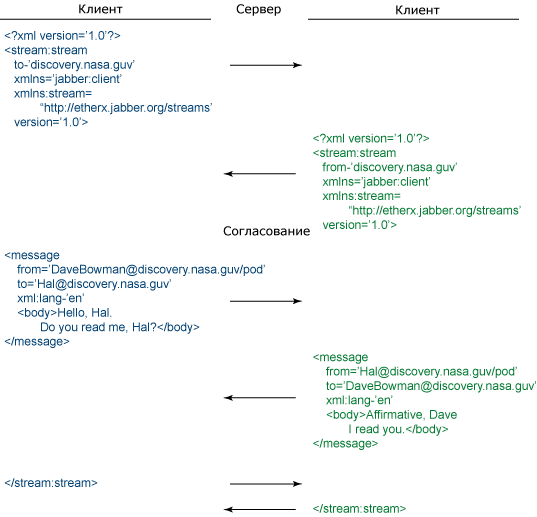
\includegraphics[width = 4cm]{images/1234.png} 
\caption{Упрощенный пример взаимодействия по протоколу XMPP}
\label{fig:baseXmpp}
\end{figure}

Далее в XML-потоке, показанном на \ref{fig:baseXmpp}, следует передача сообщений. Данное взаимодействие выполняется при помощи станс, включающих XMPP-адреса отправителя и получателя (атрибуты from и to), информацию об используемом языке, а также сами сообщения. Получив сообщение, клиент отправляет ответную стансу, изменив соответствующим образом адреса XMPP. Наконец, XML-поток закрывается путем передачи специального терминального сообщения обоими клиентами.

В процессе обмена клиент может отправить сообщение об ошибке, показанное ниже. Оно говорит о том, что второй клиент некорректно инициировал XML-поток или передал некорректную XML-стансу.

Несмотря на \ref{fig:hist} всю простоту обмена, продемонстрированного в данном примере, несложно представить, как стансы могут быть преобразованы в сообщения RPC, включающие необходимую информацию о безопасности, определенную в процессе инициирования обмена. Вместо пользователей можно использовать функции, регистрируя их в качестве узлов для создания динамической инфраструктуры Web-сервисов.


\chapter{chapter2}
\section{ваыаыв авыа ыва аыв}
\subsection{выавыаывавыа}
\subsubsection{fkdsmfksdm выьлаьывлаьвылаыва}
выавыавыаыва ыва ыва выа ыва ауца екпкуп
куп куп п укп укп укп п уп п укпукп
пуп  пк пукп укп укп укп ку пуп укпуп укп
п укп куп куп укп укп
\begin{figure}[!ht]
\centering

\includegraphics[width = 4cm]{images/123.jpeg} 
\caption{Подпись к картинке}
\label{fig:hist}
\end{figure}
ыватлдыввыа ыва выа ыва вы


\chapter{chapter3}
\section{ваыаыв авыа ыва аыв}
\subsection{выавыаывавыа}
\subsubsection{fkdsmfksdm выьлаьывлаьвылаыва}
выавыавыаыва ыва ыва выа ыва ауца екпкуп
куп куп п укп укп укп п уп п укпукп
пуп  пк пукп укп укп укп ку пуп укпуп укп
п укп куп куп укп укп

ыватлдыввыа ыва выа ыва вывыавыавыаыва ыва ыва выа ыва ауца екпкуп
куп куп п укп укп укп п уп п укпукп
пуп  пк пукп укп укп укп ку пуп укпуп укп
п укп куп куп укп укп

ыватлдыввыа ыва выа ыва вывыавыавыаыва ыва ыва выа ыва ауца екпкуп
куп куп п укп укп укп п уп п укпукп
пуп  пк пукп укп укп укп ку пуп укпуп укп
п укп куп куп укп укп

ыватлдыввыа ыва выа ыва вывыавыавыаыва ыва ыва выа ыва ауца екпкуп
куп куп п укп укп укп п уп п укпукп
пуп  пк пукп укп укп укп ку пуп укпуп укп
п укп куп куп укп укп

ыватлдыввыа ыва выа ыва вы

\subsection{выавыаывавыа}
\subsubsection{fkdsmfksdm выьлаьывлаьвылаыва}
выавыавыаыва ыва ыва выа ыва ауца екпкуп
куп куп п укп укп укп п уп п укпукп
пуп  пк пукп укп укп укп ку пуп укпуп укп
п укп куп куп укп укп

\begin{equation}
\Re{z} =\frac{n\pi \dfrac{\theta +\psi}{2}}{
\left(\dfrac{\theta +\psi}{2}\right)^2 + \left( \dfrac{1}{2}
\log \left\lvert\dfrac{B}{A}\right\rvert\right)^2}.
\end{equation}

\begin{equation}
\biggl[\sum_i a_i\Bigl\lvert\sum_j x_{ij}\Bigr\rvert^p\biggr]^{1/p}
\end{equation}

\begin{equation}
\frac{{\displaystyle\sum\nolimits_{n> 0} z^n}}
{{\displaystyle\prod\nolimits_{1\leq k\leq n} (1-q^k)}}
\end{equation}
\begin{equation}
z = \sqrt{(1 + \frac{x}{1 + \frac{c}{1 + \frac{b}{1+d}}})^2+y^2}
\end{equation}

\begin{equation}
\underbrace{\overbrace{a+b+c}^6
\cdot \overbrace{d+e+f}^9}
_\text{meaning of life} = 42
\end{equation}

\begin{equation}
P = \frac{\displaystyle{
\sum_{i=1}^n (x_i- x)
(y_i- y)}}
{\displaystyle{\left[
\sum_{i=1}^n(x_i-x)^2
\sum_{i=1}^n(y_i- y)^2
\right]^{1/2}}}
\end{equation}

ыватлдыввыа ыва выа ыва вы
выавыавыаыва ыва ыва выа ыва ауца екпкуп
куп куп п укп укп укп п уп п укпукп
пуп  пк пукп укп укп укп ку пуп укпуп укп
п укп куп куп укп укп

ыватлдыввыа ыва выа ыва вы
выавыавыаыва ыва ыва выа ыва ауца екпкуп
куп куп п укп укп укп п уп п укпукп
пуп  пк пукп укп укп укп ку пуп укпуп укп
п укп куп куп укп укп


ыватлдыввыа ыва выа ыва вы
выавыавыаыва ыва ыва выа ыва ауца екпкуп
куп куп п укп укп укп п уп п укпукп
пуп  пк пукп укп укп укп ку пуп укпуп укп
п укп куп куп укп укп

ыватлдыввыа ыва выа ыва вы
выавыавыаыва ыва ыва выа ыва ауца екпкуп
куп куп п укп укп укп п уп п укпукп
пуп  пк пукп укп укп укп ку пуп укпуп укп
п укп куп куп укп укп

ыватлдыввыа ыва выа ыва вы
выавыавыаыва ыва ыва выа ыва ауца екпкуп
куп куп п укп укп укп п уп п укпукп
пуп  пк пукп укп укп укп ку пуп укпуп укп
п укп куп куп укп укпвыавыавыаыва ыва ыва выа ыва ауца екпкуп
куп куп п укп укп укп п уп п укпукп
пуп  пк пукп укп укп укп ку пуп укпуп укп
п укп куп куп укп укпвыавыавыаыва ыва ыва выа ыва ауца екпкуп
куп куп п укп укп укп п уп п укпукп
пуп  пк пукп укп укп укп ку пуп укпуп укп
п укп куп куп укп укпвыавыавыаыва ыва ыва выа ыва ауца екпкуп
куп куп п укп укп укп п уп п укпукп
пуп  пк пукп укп укп укп ку пуп укпуп укп
п укп куп куп укп укпвыавыавыаыва ыва ыва выа ыва ауца екпкуп
куп куп п укп укп укп п уп п укпукп
пуп  пк пукп укп укп укп ку пуп укпуп укп
п укп куп куп укп укпвыавыавыаыва ыва ыва выа ыва ауца екпкуп
куп куп п укп укп укп п уп п укпукп
пуп  пк пукп укп укп укп ку пуп укпуп укп
п укп куп куп укп укпвыавыавыаыва ыва ыва выа ыва ауца екпкуп
куп куп п укп укп укп п уп п укпукп
пуп  пк пукп укп укп укп ку пуп укпуп укп
п укп куп куп укп укпвыавыавыаыва ыва ыва выа ыва ауца екпкуп
куп куп п укп укп укп п уп п укпукп
пуп  пк пукп укп укп укп ку пуп укпуп укп
п укп куп куп укп укпвыавыавыаыва ыва ыва выа ыва ауца екпкуп
куп куп п укп укп укп п уп п укпукп
пуп  пк пукп укп укп укп ку пуп укпуп укп
п укп куп куп укп укпвыавыавыаыва ыва ыва выа ыва ауца екпкуп
куп куп п укп укп укп п уп п укпукп
пуп  пк пукп укп укп укп ку пуп укпуп укп
п укп куп куп укп укпвыавыавыаыва ыва ыва выа ыва ауца екпкуп
куп куп п укп укп укп п уп п укпукп
пуп  пк пукп укп укп укп ку пуп укпуп укп
п укп куп куп укп укпвыавыавыаыва ыва ыва выа ыва ауца екпкуп
куп куп п укп укп укп п уп п укпукп
пуп  пк пукп укп укп укп ку пуп укпуп укп
п укп куп куп укп укп

ыватлдыввыа ыва выа ыва вы

\end{document}